\documentclass{article}
\usepackage{longtable}
\usepackage{graphicx}
\usepackage{booktabs}% http://ctan.org/pkg/booktabs
\usepackage{xcolor}
\newcommand{\tabitem}{~~\llap{\textbullet}~~}
\newcommand\mytodo[1]{\textcolor{red}{#1}}
\usepackage{array}
\usepackage[style=numeric,backend=bibtex]{biblatex}
\usepackage{caption}
\usepackage{amsmath}

\bibliography{Parking}

\begin{document}

\title{SoNah Parking Analytics \\ \large (working title)}
\author{Andrei Ionita}

\maketitle

\section{Introduction}
\subsection{sonah}
Looking for a parking spot has increasingly become a difficult affair for drivers. Modern navigation systems are missing a component that informs about available parking. Not only would drivers benefit from this piece of information when delivered in real time, but receiving it in advance would ensure a better planned trip, without unnecessary time being lost or by causing additional traffic.

\textbf{sonah} is an Parking Information System that provides both real-time and in advance parking information. Its vision is to integrate with navigation systems and guide the driver to its final parking position, overcoming the problem of on-street fluctuating parking places.

\subsection{Conventions}
The following terms will be used throughout this document:
\begin{itemize}
\item \textbf{parking spot} - a single parking place
\item \textbf{parking location} - a space consisting of multiple parking spots
\end{itemize}

\section{Data Acquisition}
Data is certainly ``the meat'' of any Information System. It can broadly be split into two parts: direct parking- and contextual data. The former consist generally of parking snapshots, i.e. parking situations at a certain moment in time, e.g. 71 parking spots are now free, parking spot \#42 got occupied at 17:00. Contextual data refer to the geographical infrastructure where parking locations are represented, i.e. type of parking (free, for customers, for employees), ``forbidden parking'' spots, relevant businesses in the area that lead to parking occupancy, etc.

\subsection{Parking-Data Snapshots}
\label{parking-data-snapshots}
\begin{enumerate}
\item \textbf{Sensor Data} --- the optical sensors deliver data records consisting of status change per parking spot; the format is: location (latitude, longitude), timestamp and parking spot status
\item \textbf{Parking Meter Data} --- consists of the number of tickets that have been purchased in a time period, e.g. day; this number alone does not offer direct information about the total number of parked vehicles during the certain time period, i.e. cars with permanent permission are not included, neither ticket dodgers
\item \textbf{Car Park Data} - the current number of free parking spaces in the city car parks as they are made available online
\end{enumerate}

\subsection{Parking Geographical Information}
\label{parking-geo-info}
\begin{enumerate}
\item \textbf{Open Street Map} ---- OSM is an open Geographical Information System (GIS) platform where content is contributed by users. OSM is able to store detailed parking information, among others, consisting of location, type of parking (public, customers, company, etc.), parking fee, parking capacity, and others attributes.
\item \textbf{User-Generated Data} --- a smartphone application that asks users to introduce pieces of information regarding parking areas at their convenience, e.g. disabled parking spots, number of current free parking spots, type of business in the building nearby etc. Some of the information asked for is intentionally redundant, in order to cross-validate data from other sources. The app users will hence have a stake at improving the parking-related infrastructure. 
\end{enumerate}

\subsection{Other contextual information}
\label{other-context-info}
\begin{enumerate}
\item \textbf{Events} --- whether concerts, sporting events, Christmas markets or others, events can greatly impact parking occupancy for certain periods of time. Therefore it makes sense to gain access to the time and place of events.
\item \textbf{Weather Conditions} --- dry, rainy or snowy weather plays a large role when deciding to use a car in the city and hence impacts parking as well.
\item \textbf{Traffic Flow / Construction Sites} --- investigating the correlation between high/low traffic and nearby parking locations may help in improving parking prediction. It is therefore important to gain access to traffic flow data and temporary construction site locations.
\end{enumerate}

\subsection{Access to Data}
\label{sec:access-to-data}
As soon as we discover a useful data source, gaining access to it is essential. Internal data will be saved in our \textbf{database}s. In case of Parking Snapshots, a NoSQL database will be used, since snapshots are committed very frequently and non-relationality offers the advantage of easier processing, i.e. by using map/reduce, etc. Static data like geographical infrastructure shall conveniently be stored inside a relational database, since its size and rate of change pose no issues for processing.

A challenge here is modeling the parking areas. Since there are no clearly defined limits for a parking areas, i.e. neither are parking meters used by the drivers necessarily the closest to their parking position, nor is this distance trivial to define, we will organise parking areas according to the business or institutions in that area. Hence all parking spots belonging to a restaurant are a unit, the same for school parking spots, office parking spots, and so on. These parking layers may overlap (see Figure~\ref{fig:parking-layers}).

\begin{figure}[!ht]
    \centering
    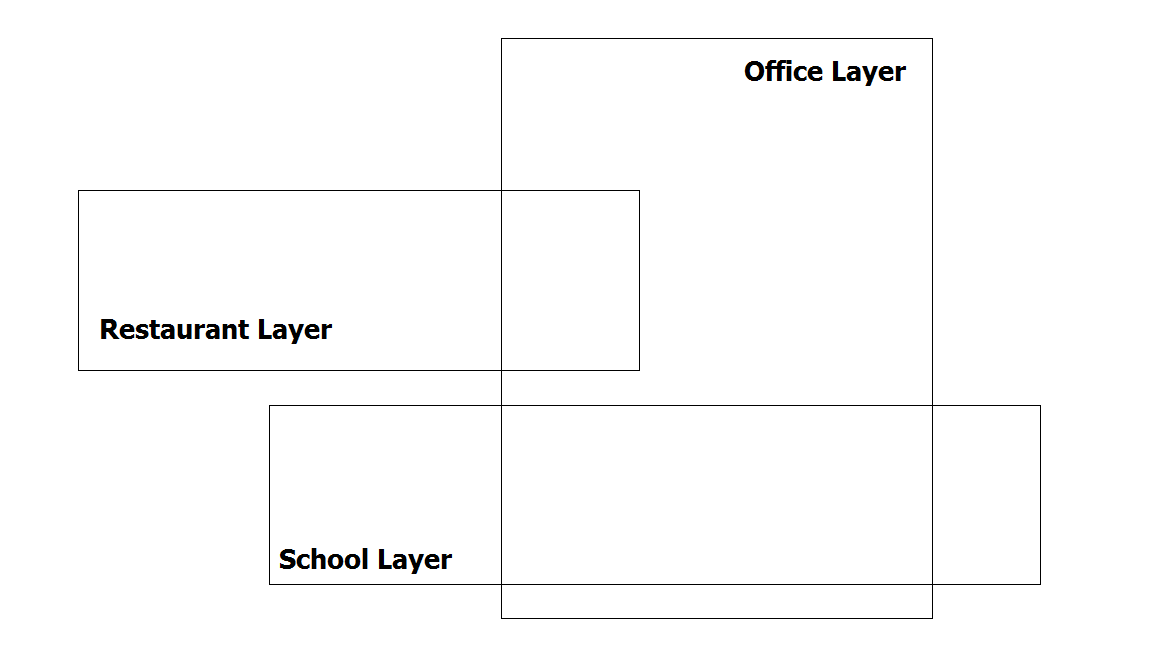
\includegraphics[width=3.0in]{ParkingLayers}
    \caption{Parking Locations organised in layers according to business and institutions on site}
    \label{fig:parking-layers}
\end{figure}

External data is at best accessed via an \textbf{Application Programming Interface (API)}, preferably REST, since this paradigm simplifies HTTP request/response processing; nevertheless, we accept querying other kinds of APIs too.

When external information is not explicitly made available, we investigate the approach of \textbf{crawling} or scraping the providers' web-sites. Scraping is the process in which regular expressions are matched against retrieved HTML content in order to ``clip out'' interesting information. Before any external party content is retrieved however, we will make sure to comply with the law in this respect and will check whether the certain web-sites are crawlable at all.

\subsection{Data Coverage Limitations}
In spite of all the previously described different data sources at our disposal, there will be significant numbers of parking locations that will not be covered. Therefore, we investigate extrapolating the already available data to the unsupervised parking locations, i.e. extend and adapt values from one location to another by taking into account contextual information (see~\ref{parking-geo-info} and~\ref{other-context-info}). More on this shall be discussed in the Model Selection section of the thesis.

\vspace{2mm}
To summarize all data sources, Table~\ref{tab:data-overview} presents an overview of the comprised data and its characteristics.

\begin{table}
	\resizebox{\textwidth}{!}{
	\centering
    \begin{tabular}{ | c | c | c | c | c |}
    \hline
    \textbf{Data type}& \textbf{Object reported} & \textbf{Timestamp} & \textbf{Retrieval cycle} & \textbf{Access}  \\ \hline
    \textbf{Sensors} & parking spot & live & immediately & database \\ \hline
    \textbf{Parking Meters} & parking ticket & historical & periodically & API \\ \hline
	\textbf{Car Parks} & vehicle & live & periodically & crawling \\ \hline
	\textbf{OSM} & GIS element & --- & periodically & API \\ \hline
    \textbf{User-generated} & anything & --- & immediately & database \\ \hline
	\textbf{Events} & event element & near future & periodically & crawling \\ \hline
	\textbf{Weather} & weather element & near future & periodically & crawling/API \\ \hline
	\textbf{Traffic flows} & traffic report & live & periodically & crawling/API \\ \hline
    \end{tabular}}
	\caption{Data overview and its features}
    \label{tab:data-overview}
\end{table}

\section{Modeling parking locations}
\subsection{Feature selection}
In order to better describe the model, we first need to determine its relevant features, i.e. parameters that correlate with the parking availability outcome. Common features include time of day, day of week and events\cite{Caicedo}\cite{Chen}\cite{Hoessinger2014}. Weather conditions may also play a role, which we shall investigate. Further, we shall look into the presence relevant buildings or geo-features in the neighborhood, i.e. offices, schools, residential areas, etc. that provide parking areas and account for certain parking behaviors.

\subsection{Measuring accuracy}
We need some metrics in order to evaluate the performances of the following models. Given a time series 
$y(t), t=1,..,n$ representing observed values, and its predicted series $\hat{y}(t)$, the Mean Absolute Percentage Error is defined as \cite{Chen}\cite{Rajabioun}

$$MAPE(y, \hat{y}) = \frac{1}{n}\sum_{i=1}^{n}|\frac{y(t) - \hat{y}(t)}{y(t)}|$$

\subsection{Model selection}
We shall present methods that have been applied in the relevant literature for problems similarly defined as ours. Each section consists of a short definition of the method and points out its hallmarks and the reasons for which it applies in our setting. The thesis may go into some further degree of relevant mathematical detail.

\subsubsection{Linear Regression (OLS)}
Linear Regression models suppose that the predicted time series is a linear combination of defined attributes. Considering $y(t)$ as a time series, $f_i(t)$ the value of the feature $i$ at time $t$, its estimation is given by:

$$y(t) = w_0 + \sum_{i=1}^{|features|}w_i f_i(t) + \epsilon(t)$$

where $w_i$ are weights determined during training and $\epsilon(t)$ is the least square error that results from optimally fitting the line to the points in the graph (see Figure~\ref{fig:linear-regression}).

\begin{figure}[!ht]
    \centering
    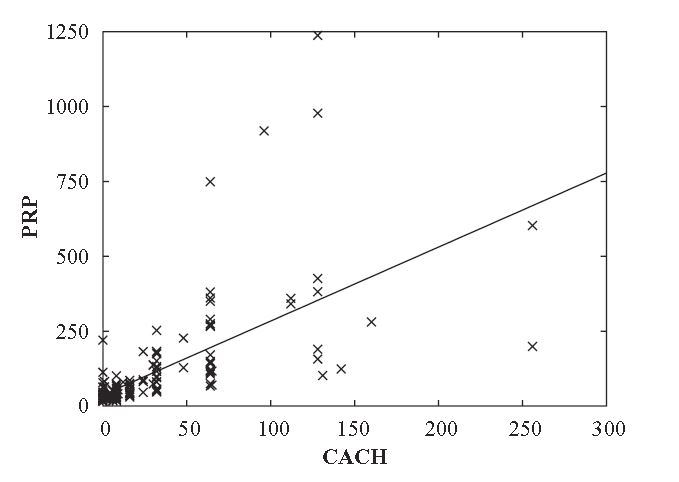
\includegraphics[width=3.0in]{linear-regression}
    \caption{Example of a line that fits a set of points according to linear regression; plot taken from \cite{Witten} }
    \label{fig:linear-regression}
\end{figure}


\vspace{2mm}
Chen\cite{Chen} tries out a linear regression model for 120 parking spots and 1 hour ahead prediction. His $R^2$ value is 92\% and MAPE is close to 8\%.

\subsubsection{Support Vector Regression (SVR)}
Support Vector Regression is a prediction method applicable also for non-linear models. Compared to linear regression, it distinguishes itself by fitting future points using a non-linear combination of support vectors, i.e. selected points from the current set. During the training phase, the support vectors are selected as the points that fall outside the $\epsilon$ error value range (see Figure~\ref{fig:svr}). The error is measured in absolute value and only accounts for points outside the $2\epsilon$ range. 

$$x = b + \sum_{i\:support\:vector} \alpha_i (a(i) \cdot a)  $$
where $b$ and $\alpha_i$ are determined in the training phase, $a(i)$ are the support vectors and $a$ is the current instance.  The dot product term is called the kernel function and is responsible for non-linear behavior when it contains higher order factors. There are various kernel functions used and choosing a good one for one's case is not trivial. As a whole, the algorithm tends to both minimize the error and simultaneously to maximize the flatness of the regression function, thus avoiding overfitting, i.e. biasing the model towards the training data.

\begin{figure}[!ht]
    \centering
    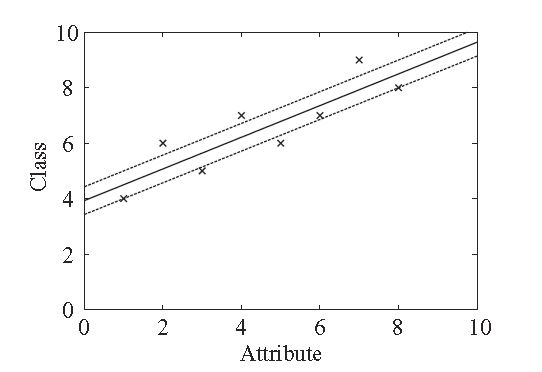
\includegraphics[width=3.0in]{svr}
    \caption{Example of a line determined by SVR; some points lie outside the $2\epsilon$-wide band; plot taken from \cite{Witten} }
    \label{fig:svr}
\end{figure}

\vspace{2mm}
Chen\cite{Chen} constructs vectors of 24 elements that represent parking values corresponding to the last 24 hours and uses Support Vector Regression to predict future values:

$$y(t+1) = w^T\gamma(x_k(t)) + b$$
where $x_k(t)$ holds the parking data for $y(t-k+1), y(t-k+2), ..., y(t)$. The application of this model yields a MAPE value of about 7\% for about 100 parking spots.

\subsubsection{ARIMA}
In time series analysis autoregressive integrated moving average (ARIMA), models are used to forecast future points in the series. The autoregressive (AR) part accounts for its own lagged (i.e. previous) values, while its moving average (MA) part computes future values using past prediction errors. An ARIMA model predicts future values using its both components. Its prerequisite is that the data has to be stationary, i.e. its mean and variance are constant over time. In order to achieve that, the time series at hand may be differentiated (i.e. replace current point with the difference to its previous point) more times.

$ARIMA(p,d,q)$ stands for a model that has been differentiated $d$ times, looks behind at its last $p$ values and at its previous $q$ prediction errors. An $ARIMA(p,d,q)(P,D,Q)_m$ is a seasonal model that recognizes some temporary behavior based on reoccurring events of period $m$.

\vspace{2mm}
Chen\cite{Chen} uses an $ARIMA(2,0,1) x (1,1,0)_{24}$ model with the seasonal factor corresponding to the hours of the day. He measures a MAPE error ratio for 100+ parking spots for 1 hour ahead of about 6\%.

\vspace{2mm}
Rajabioun and Ioannou\cite{Rajabioun} propose a multivariate autoregressive model that takes into account not only temporal but also spatial correlations of parking availability. They observe that the nearer the parking spots are, the more similar the occupancy rates are. Their model yields a 14\% MAPE for a 20-minute prediction horizon.

\subsubsection{Neural Networks}
\label{sec:neural-networks}
Neural Networks (NN) relax the conditions of linearity and stationarity that the previous models impose and hence may achieve new levels of accuracy. They consists of a directed graph that contains nodes (i.e. neurons) with a  activation function, which map inputs to output values. In particular, Multilayer Perceptrons (MLP) are models where the activation function is non-linear. Apart from the input and output layers, MLPs have one or more hidden layers. Learning occurs by changing the weights in the activation functions by observing the error between the output and expected result. This supervised learning method is called backpropagation.

\vspace{2mm}
Vlahogianni et al.\cite{Vlahogianni} use a MLP with 8 hidden layers for a 4\% MAPE 1 hour prediction error. Chen\cite{Chen} achieves a 3\% error when using 2-hidden layer NN for an 1 hour-ahead prediction.

\subsubsection{Continuous Markov Chains}
Markov Chains are used to model processes in which future states depend causally only on the current state and not on previous states. Between any two states there may be a transition probability which expresses how likely the process is to jump from one state to the other. Markov Chains can be either discrete- or continuous-time. For the latter, the time spent in each state has an exponential distribution, i.e. states transitions at fixed time intervals.

\vspace{2mm}
This model's prerequisites seem to apply to the parking space occupation problem: future parking configurations indeed depend solely on the current configuration. Caliskan et al.\cite{Caliskan2007} defines a state of the process by the absolute occupancy value. The authors consider the average parking arrival rate and the average parking rate (i.e. inverse of parking duration) to construct a Continuous-Time Markov Chain (CTMC) and to predict future occupancy values. In Figure~\ref{fig:markov-chain}, the CTMC is represented by $\lambda$ (parking arrival rate) and $\mu$ (parking rate). The authors do not provide an exact error measure for their application of the model, however state that ``our prediction algorithm is most effective for prediction times up to 15 minutes [..] with increasing prediction time, the uncertainty of the model increases''.

\begin{figure}[!ht]
    \centering
    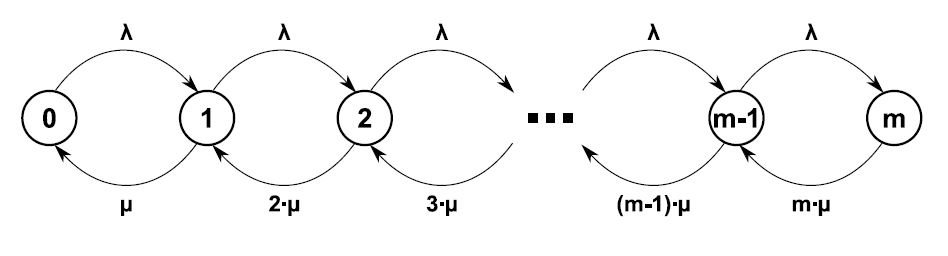
\includegraphics[width=4.0in]{markov-chain}
    \caption{Continuous-Time Markov Chain corresponding to a Parking Location; taken from \cite{Caliskan2007}}
    \label{fig:markov-chain}
\end{figure}

To summarize the presented methods, we outline their main features in Table~\ref{tab:methods}. An exact error-comparison based on the same testing ground is, at this point, not available. Individual testing results have been provided in corresponding methods' paragraphs.

%\bgroup
%\def\arraystretch{1.5}%  1 is the default, change whatever you need
{\footnotesize
\begin{table}[!ht]
 \centering
 {\renewcommand{\arraystretch}{2.5}
	\resizebox{\textwidth}{!}{
  \begin{tabular}{ | c | c | c | }
    \hline
    \textbf{Method} & \textbf{Recommending features} & \textbf{Limitations} \\ \hline
    \textbf{Linear Regression} & \begin{minipage}{0.4\textwidth} general and simple prediction method \end{minipage} & \begin{minipage}{0.4\textwidth} only matches linear models \end{minipage} \\ \hline
    \textbf{SVR} & \begin{minipage}{0.4\textwidth} additionally fits non-linear models \end{minipage} & \begin{minipage}{0.4\textwidth}difficulty choosing kernel function\end{minipage} \\ \hline
    \textbf{ARIMA} & \begin{minipage}{0.4\textwidth} applies directly to time-series \end{minipage} & \begin{minipage}{0.4\textwidth}requires linearity and stationarity \end{minipage} \\ \hline
	\textbf{Neural Networks} & \begin{minipage}{0.4\textwidth}adaptable to latest observed results via backpropagation \end{minipage} & \begin{minipage}{0.4\textwidth} proneness to overfitting; its ``black box'' nature \end{minipage} \\ \hline
	\textbf{Markov Chains} & \begin{minipage}{0.4\textwidth} models processes of independent events\end{minipage} & \begin{minipage}{0.4\textwidth}does not accommodate other features than time-related ones \end{minipage}\\ \hline
  \end{tabular}}}
	\caption{Prediction Method Summary}
 	\label{tab:methods}
\end{table}}
%\egroup

 
\section{Implementation}
The implementation will be done at SoNah UG. The software component will be realised in Java or Python. It remains to be decided whether it will take the form of a library or will integrate with the User-Interface in an MVC application (e.g. in Django). Databases used will be a NoSQL (e.g. MongoDB) and a relational database (e.g. MySQL).

\subsection{Evaluation}
A fraction of the accumulated live parking data will be used towards training the model. We estimate to use  10-30\% of the data for testing, depending on how consolidated the model already is.

\vspace{2mm}
Alternatively, test data can be simulated, in case not enough parking data was collected by that time.

\section{Research Goals}
In order to arrive at an efficient parking prediction application, there are several unknowns that need to be investigated. The thesis will elaborate answers to the following questions.

\vspace{2mm}
\textbf{How are the data stored and retrieved?}\\
As outlined in~\ref{sec:access-to-data}, data is either stored internally or accessed from external sources. The former is split among dynamic and static data. Dynamic data are mainly represented by sensor data records and are expected to be uploaded in frequent intervals. NoSQL databases are suited for this particular case, as inbuilt retrieval and aggregation operations are available, e.g. map/reduce. How efficient will this turn out in practice, will be reflected in the application performance.

\vspace{2mm}
\textbf{How are parking- and contextual data associated?}\\
Both parking- and contextual information (GIS, traffic, events, etc.) have a geographical position in common, around which data can be linked. How efficient will the association be saved and retrieved, the thesis will provide answers.

\vspace{2mm}
\textbf{What features are indeed relevant in order to build a prediction model with?}\\
A feature (e.g. business surroundings, weather, traffic) can be considered relevant to a prediction model if it has a mathematical influence on the parking occupancy values, i.e. if a correlation with the end-values can be determined. Whether all the considered data in this proposal is indeed relevant, or other features will be found to be relevant (~\ref{parking-data-snapshots}, ~\ref{parking-geo-info} and ~\ref{other-context-info}), it remains to be seen.

\vspace{2mm}
\textbf{In what degree can ``parking profiles'' be extrapolated to fit unsupervised parking locations?}\\
The degree in which extrapolation of parking information and contextual elements is possible will depend on the results of the prediction models. The data first will be tested on areas for which there are data sources, so that the results can be cross-validated. Whether the validation will be positive, we expect to find out.

\vspace{2mm}
\textbf{How accurate can a system predict availability of free parking spots?} \\
There have been related investigations that yield results as good as \%3 MAPE for 1-hour in advance prediction(see~\ref{sec:neural-networks}). The results of our work will be measured on the same scale and will be compared to existing research. It is still to be seen whether our results will improve on those with a similar setup.

\vspace{2mm}
\textbf{What additional conditions should a parking recommending system take into account?} \\
Apart from rate of free parking spots in parking locations, another relevant condition may be minimizing the distance towards the final destination of drivers, i.e. home, work, restaurant. How a trade-off between multiple optimization functions can be achieved and possibly other conditions, will be further investigated.

\section{Timetable}
(to be filled in)

\nocite{*}

\printbibliography

\end{document}